\documentclass[a4paper, 14pt]{extarticle}
\usepackage{indentfirst}
\usepackage[T2A]{fontenc}
\usepackage[utf8]{inputenc}
\usepackage[english, russian]{babel}
\usepackage{amsmath, amssymb, amsthm, amscd, latexsym}
\usepackage{graphicx, caption}
\usepackage[left=3cm,right=2cm,top=2cm,bottom=3cm]{geometry}
\setlength{\parindent}{1.25cm}
\linespread{1.25}
\graphicspath{{pictures/}}

\usepackage{hyperref}
\hypersetup{
    colorlinks=true,
    linkcolor=blue,
    filecolor=magenta,      
    urlcolor=cyan,
    pdfpagemode=FullScreen,
}


\title{Проблема выразимости бинарных нейронных сетей}
\author{Р.\,С.~Мурадасилов}
\date{2020}

\begin{document}
\begin{titlepage}
\begin{center}
        
\textbf{Филиал Московского Государственного Университета\\
имени М.В. Ломоносова в г. Ташкенте} \vskip 0.3cm
\textbf{Факультет прикладной математики и информатики} \vskip 0.3cm
\textbf{Кафедра прикладной математики и информатики} \vskip 3cm
            
\textbf{Мурадасилов Руслан Серверович} \vskip 1cm
            
\textbf{КУРСОВАЯ РАБОТА} \vskip 1cm
            
\normalsize { \textbf{на тему: \guillemotleft Проблема выразимости бинарных нейронных сетей\guillemotright \\ \vskip 0.5cm
по направлению 01.03.02 \guillemotleft Прикладная математика и информатика\guillemotright} }
\vskip 1.5cm
\end{center}

\begin{flushleft}
Курсовая работа рассмотрена и рекомендована к защите \vskip 5pt
зав.кафедрой <<ПМиИ>>, д.ф.-м.н., профессор \rule{2.365cm}{0.5pt} Кудрявцев В.\,Б.
\end{flushleft}
\begin{flushleft}
Научный руководитель:\vskip 5pt
к.ф.-м.н. \rule{10.798cm}{0.5pt} Иванов И.\,Е.
\end{flushleft}
          
\begin{flushright}
<<\rule{1cm}{0.5pt}>>\rule{3.5cm}{0.5pt} 2020 г.
\end{flushright}
        
\vfill   
\begin{center}
Ташкент 2020
\end{center}
\end{titlepage}


\begin{abstract}
    В данной работе рассматривается проблема выразимости бинарной нейронной сети. Определено, как устроен слой такой нейронной сети. Исследуется полнота слоя при ограничениях. Обозначена проблема аппроксимации булевых функций линейными булевыми функциями.
\end{abstract}

\begin{abstract}
In this work
\end{abstract}


\setcounter{page}{2}
\newpage
\tableofcontents
\newpage


\section{Введение}
    В данной работе рассматривается проблема выразимости бинарной нейронной сети. Вводятся понятия, определяющие структуру слоя. Рассматривается проблема полноты нейронной сети, слой которой представляет собой комбинацию <<линейная функция + некоторая нелинейность>>. Доказано, что такая нейронная сеть будет полна. Также доказано существование полной нейронной сети при ограничении в два слоя.
    
    Ставится задача исследовать аппроксимацию булевых функций нейронной сетью, слой которой состоит только из линейных функций.
\newpage


\section{Историческая часть вопроса}
    За последнее десятилетие сложность и способности нейронных сетей существенно выросли, однако их потенциал до сих пор ограничивают стоимость и энергия потребления. Как известно, нейронные сети состоят из нескольких слоев взвешенных сумм, которые предсказывают нужный результат. Хранение всех значений чисел с плавающей запятой значительно увеличивает время обучения и требует большое количество памяти, что вызывает необходимость использовать только специальное оборудование, которое выдержит подобную нагрузку.
    
    Чтобы устройство с ограниченными ресурсами могло решать такие проблемы глубокого обучения, как распознавание лиц в реальном времени, необходимо использовать в качестве весов бинарные числа, а в качестве функций активации "--- бинарные аналоги функций активации в непрерывном случае, то есть <<бинаризовать>> нейронную сеть. Это позволит хранить гораздо больший объем данных, используя, например, 32-битный контроллер. Использование битовых операций сокращает время исполнения. Размеры бинарных нейронных сетей намного меньше, чем у их вещественнных аналогов. Точность моделей также меньше, но эта разница в точности постепенно сокращается и бинарные нейронный сети становятся точнее на больших датасетах, как ImageNet.
    
    Идея бинарной нейронной сети была впервые предложена Matthieu Courbariaux, где веса и функции активации используют только бинарные числа как и в inference, так и в алгоритме обратного распространения ошибки с использованием метода градиентого спуска (SGD) \hyperlink{p1}{[1]}.
    
    Чуть позже Mohammad Rastegari в модели XNOR-Net \hyperlink{p2}{[2]} добавляет gain term, чтобы компенсировать потерю информации во время бинаризации, который был получен из статистики весов и функций активации до бинаризации. Это улучшило общие показатели, но подсчет gain term оказался дорогостоящим.
    
    Victor Zhou попытался обобщить квантизацию и использовал преимущество битовых операций для фиксированной точки данных, варьируя ее размерность \hyperlink{p3}{[3]}. Zhou представил DoReFa-Net, модель с переменной размерностью весов, функций активации и даже вычисления градиента во время обратного распространения ошибки со значительно улучшенным временем обучения.
    
    Другие модели также добились положительных результатов. Zheng Tang ускорил время обучения, изучив как влияет скорость обучения на показатели нейронной сети и на колеблемость бинарных значений \hyperlink{p4}{[4]}. Идея BNN+, созданная Sajad Darabi,также улучшает скорость обучения, использую другую эффективную функцию обратного распространения вместо импульсной \hyperlink{p5}{[5]}.
    
    Сравнение результатов всех этих моделей на разных датасетах были подробно описаны в работе Taylor Simons и Dah-Jye Lee \hyperlink{p6}{[6]}. Наглядно видно, что на MNIST, SVHN, CIFAR и ImageNet датасетах бинарные нейронные сети практически не уступают своим вещественнным аналогам.
    
    В данной работе рассматривается вопрос полноты бинарной нейронной сети, то есть способность в точности выразить булеву функцию. А также ставится задача аппроксимации булевых функций, то есть способность выразить булеву функцию с некоторой допустимой погрешностью. С практической точки зрения устраивают оба варианта.
\newpage


\section{Основные результаты}
\subsection{Полнота}
    Введем основные определения.
    
    \textbf{Определение 1.} \emph{Нейронной сетью} называются композиции функций, каждую из которых назовем слоем. Под композицией функций понимается подстановка одной функции в качестве аргумента другой.
    
    \textbf{Определение 2.} \emph{Слоем} называется композиция весовой функции и нелинейного бинарного оператора, выступающего в роли функции активации. \emph{Входным слоем} будем называть вектор $X = (x_1, ... x_n)\in \{0, 1\}^n$, а \emph{выходным} "--- вектор $Y = (y_1, ... y_n)\in \{0, 1\}^n$.
    
    \textbf{Определение 2.} \emph{Весовой функцией} называется линейная булева функция, применяемая ко всем выходам предыдущего слоя, включая входной слой.
    
    \textbf{Определение 3.} Вектор $f^i = (f^i_1, ..., f^i_k)$, где i "--- номер скрытого слоя, k "--- количество нейронов внутри i-ого слоя, а каждая $f^i_j$ является функцией алгебры логики от n переменных $(j = \overline{1, k})$ называется \emph{бинарным оператором}.
    
    \textbf{Определение 4.} Бинарный оператор называется \emph{линейным}, если каждая его компонента $f^i_j$ является линейной $(j = \overline{1, k})$. Соответсвенно, бинарный оператор называется \emph{нелинейным}, если хотя бы одна из его компонент $f^i_j$ является нелинейной $(j = \overline{1, k})$.
    
    Справедлив следующий результат, относящийся к проблеме полноты бинарной нейронной сети с такой архитектурой.
    
    \textbf{Теорема 1.}
    Бинарная нейронная сеть с линейной булевой весовой функцией и нелинейным бинарным оператором в роли функции активации полна в $P_2$.
    
    \textbf{Доказательство.}
    Так как класс булевых линейных функций является предполным, то достаточно хотя бы одной нелинейной функции, чтобы нейронная сеть могла порождать $P_2$. По определению нелинейного бинарного оператора такая функция будет существовать, что доказывает теорему. \hfill $\blacksquare$\\
    
    Рассмотрим вопрос существования полной бинарной нейросети с двумя скрытыми слоями. Справедлива следующая теорема.
    
    \textbf{Теорема 2.}
    Существует бинарная нейронная сеть с линейной булевой весовой функцией и нелинейным бинарным оператором в роли функции активации с двумя скрытыми слоями, которая полна в $P_2$.
    
    \textbf{Доказательство.}
    Построим бинарную нейронную сеть, реализующую СДНФ функции. Нейросеть будет полносвязной, так как в СДНФ все конъюнкции полные. Во входном слое вектор $X = (x_1, ... x_n)\in \{0, 1\}^n$, на котором хотим получить значение функции. В первом скрытом слое k нейронов ($k\leqslant2^n$), реализующих эти конъюнкции, то есть $f^1 = (f^1_1, ..., f^1_k)$ $\forall f^1_j = \wedge$, $j = \overline{1, k}$. Весовая функция первого скрытого слоя "--- исключающее «или», которая позволит получать отрицания переменных при передаче их в конъюнкцию. Во втором скрытом слое один нейрон, принимающий на вход все конъюнкции СДНФ и реализующий их дизъюнкцию, то есть $f^2 = \vee$. Таким образом, функции активации (конъюнкция, дизъюнкция) — нелинейны, а весовая (исключающее «или») — линейна, и мы сохраняем структуру слоя (рис. 1).
    
    \begin{figure}[h]
    \begin{center}
    %\begin{minipage}[h]{0.2\linewidth}%
    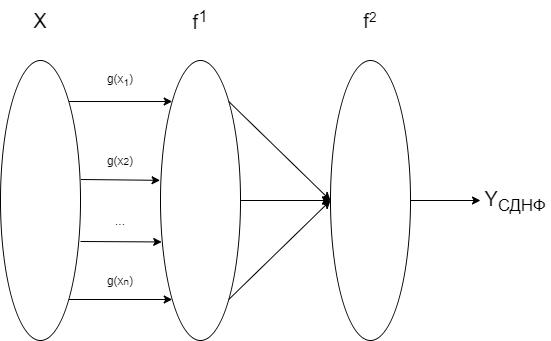
\includegraphics[width=1\linewidth]{picture1.png}
    \caption{}
    \label{ris:experimcoded}
    %\end{minipage}%
    \end{center}
    \end{figure}
    
    Так как СДНФ функции конечна и единственна, то по ней мы сможем однозначно восстановить все функции алгебры логики, и такая нейронная сеть будет полна, что и требовалось доказать. \hfill $\blacksquare$\\
    
    Исторически, проблема выразимости нейронных сетей с вещественными значениями прослеживается от 13-й проблемы Гильберта, ставящей вопрос "существует ли непрерывная функция трех переменных, которая не может быть представлена через композицию непрерывных функций двух переменных". Она была решена в 1957 г. В.А. Арнольдом; oн показал, что любая непрерывная функция трех переменных представляется в виде композиции непрерывных функций двух переменных. В том же 1957 г. А.Н. Колмогоров доказал более сильную теорему: для реализации функций многих переменных достаточно операций суммирования и композиции функций одной переменной. Эта теорема в 1987 году была переложена Хехт–Нильсеном для нейронных сетей: любая функция нескольких переменных может быть представлена двухслойной нейронной сетью с прямыми полными связями с $N$ нейронами входного слоя, $(2N+1)$ нейронами скрытого слоя с ограниченными  функциями активации (например, сигмоидальными) и $M$ нейронами выходного слоя с неизвестными функциями активации \hyperlink{p7}{[7, 8, 9, 10]}.
    
    В бинарных нейронных сетях справедлив аналогичный результат.
    
    \textbf{Теорема 3.}
    Бинарная нейронная сеть с линейной булевой весовой функцией и нелинейным бинарным оператором в роли функции активации с тремя слоями полна в $P_2$.
    
    \textbf{Доказательство.}
    
    
\subsection{Аппроксимация}   
    В практике расчетов, связанных с обработкой экспериментальных данных, вычислением $f(x)$, разработкой вычислительных методов, встречаются следующие две ситуации:
    
    \begin{enumerate}
    \item Как установить вид функции $y = f(x)$, если она неизвестна? Предполагается при этом, что задана таблица ее значений, которая получена либо из экспериментальных измерений, либо из сложных расчетов.
    \item Как упростить вычисление известной функции $f(x)$ или же её характеристик, если $f(x)$ слишком сложная?
    \end{enumerate}
    
    Ответы на эти вопросы даются теорией аппроксимации функций, основная задача которой состоит в нахождении функции $\varphi(x)$, близкой (т.е. аппроксимирующей) в некотором нормированном пространстве к исходной функции $y = f(x)$. Функцию $\varphi(x)$ при этом выбирают такой, чтобы она была максимально удобной для последующих расчетов.
    
    Одним из замечательных свойств нейронных сетей является способность аппроксимировать и, более того, быть универсальными аппроксиматорами. С помощью нейронных сетей можно аппроксимировать сколь угодно точно непрерывные функции многих переменных.
    
    Что касается бинарных нейронных сетей, здесь этот вопрос ещё хорошо не изучен. Важно доказать, насколько хорошо можно аппроксимировать любую булеву функцию линейными, то есть важен вопрос линейной аппроксимации в бинарном случае.
    
    Введем метрику, вычисляющую процент несовпадений по следующей формуле:
    $$\sum |y_{real} - y_{pred}| \cdot 100\%,$$ где $y_{real}$ "--- столбец значений предсказываемой функции, $y_{pred}$ "--- столбец значений функции, полученной в результате аппроксимации.
    
\newpage

        
\section{Заключение}
    В данной работе исследована проблема полноты бинарной нейронной сети. Доказана теорема о полноте нейронной сети со слоем <<линейная функция + некоторая нелинейность>>. Также доказан результат о существовании полной нейронной сети при ограничении в два слоя с помощью СДНФ.
    
    Обозначена важность проблемы аппроксимации булевых функций линейными функциями. Ставится цель изучить линейную аппроксимацию в бинарном случае.
\newpage


\section{Список использованной литературы}
    \hypertarget{p1}{[1]} Courbariaux, M.; Bengio, Y. BinaryNet: Training Deep Neural Networks with Weights and Activations Constrained to $+1$ or $-1$. arXiv:1602.02830.
    
    \hypertarget{p2}{[2]} Rastegari, M.; Ordonez, V.; Redmon, J.; Farhadi, A. XNOR-Net: ImageNet Classification Using Binary Convolutional Neural Networks. In Proceedings of the European Conference on Computer Vision, Amsterdam, The Netherlands, 11–14 October 2016; pp. 525–542.32.
    
    \hypertarget{p3}{[3]} Zhou, S.; Ni, Z.; Zhou, X.; Wen, H.; Wu, Y.; Zou, Y. DoReFa-Net: Training Low Bitwidth Convolutional Neural Networks with Low Bitwidth Gradients. arXiv 2016, arXiv:1606.06160.
    
    \hypertarget{p4}{[4]} Tang, W.; Hua, G.; Wang, L. How to Train a Compact Binary Neural Network with High Accuracy? In Proceedings of the Thirty-First AAAI Conference on Artificial Intelligence, San Francisco, CA, USA, 4–9 February 2017
    
    \hypertarget{p5}{[5]} Darabi, S.; Belbahri, M.; Partovi Nia, V.; Courbariaux, M. Regularized Binary Network Training. arXiv:1812.11800
    
    \hypertarget{p6}{[6]} Simons, T.; Lee, D. A Review of Binarized Neural Networks. Electrical and Computer Engineering, Brigham Young University, Provo, UT 84602, USA.
    
    \hypertarget{p7}{[7]} Колмогоров А. Н. О представлении непрерывных функций нескольких переменных суперпозициями непрерывных функций меньшего числа переменных. ДАН СССР, 1956, Т.108, №2, С. 179-182
    
    \hypertarget{p7}{[8]} Арнольд В.И. О функции трех переменных. ДАН СССР, 1957, Т.114, №4, С. 679-681
    
    \hypertarget{p7}{[9]} Колмогоров А. Н. О представлении непрерывных функций нескольких переменных в виде суперпозиций непрерывных функций одного переменного и сложения. ДАН СССР, 1957, Т.114, №5, С. 953-956
    
    \hypertarget{p7}{[10]} Hecht-Nielsen R. Kolmogorov’s mapping neural network existence theorem. IEEE First Annual Int. Conf. on Neural Networks, San Diego, 1987. Vol. 3. — P. 11—13.
 
    
\end{document}